\apendice{Documentación técnica de programación}

\section{Introducción}

En este apéndice se recoge como está estructurado el directorio del proyecto, la instalación del proyecto, la instalación del software relacionado con su funcionamiento y la creación de las \textit{builds} para su instalación en los 2 dispositivos. Serán necesarias conocimientos de C\# y estar familiarizado con Unity para realizar modificaciones del proyecto. 

Para solucionar cualquier contratiempo relacionado con el paquete de Mixed Reality Toolkit que pueda surgir en un futuro, recomiendo acudir al manual y documentación oficial del \textit{plugin} \cite{microsoft:install}.

\section{Estructura de directorios}

La estructura del directorio puede no coincidir completamente con el proyecto subido a GitHub. Esto es debido a que al ser un TFG llevado a cabo con la empresa ITCL, se ha suprimido parte del código fuente para evitar la reproducción y copia del proyecto.

El directorio del proyecto de Unity es siguiente:

\begin{itemize}
\tightlist
\item
    \textbf{/Assests} Carpeta que contiene todos los recursos del proyecto.
    \begin{itemize}
    \tightlist
    \item
        \textbf{/Assests/Materials} Materiales utilizados en el proyecto.
    \item
        \textbf{/Assests/MixedRealityToolkit.Generated} Almacena los perfiles por defecto y personalizados de MRTK.
    \item
        \textbf{/Assests/MRTK} Recursos del paquete Mixed Reality Toolkit (MRTK).
    \item
        \textbf{/Assests/Prefabs} Contiene los objetos reutilizables creados durante el desarrollo del proyecto.
    \item
        \textbf{/Assests/Scenes} Se encuentran almacenadas las dos escenas del proyecto.
    \item
        \textbf{/Assests/Scripts} Scripts que implementan las funcionalidades de la aplicación.
    \item
        \textbf{/Assests/TextMesh Pro} Carpeta que contiene el paquete de TextMesh Pro.
    \end{itemize}
\item
    \textbf{/Builds} Carpeta que contiene las \textit{builds}.
\item
    \textbf{/Library} Carpeta que contiene todas las librerías utilizadas en el proyecto.
\item
    \textbf{/Logs} Capeta que contiene un registro de todos los paquetes instalados.
\item
    \textbf{/obj} Carpeta que contiene todas las referencias del paquete MRTK.
\item
    \textbf{/Packages} Carpeta que contiene el archivo que le indica Unity los que paquetes están instalados en el proyecto, su versión y de donde provienen.
\item
    \textbf{/ProjectSettings} Carpeta que contiene la configuración del proyecto.
\end{itemize} 

\section{Manual del programador} \label{recomendados}

Para poder comenzar a desarrollar con este proyecto se necesitarán un ordenador que cumpla unas especificaciones mínimas de hardware y unas HoloLens 2. Los componentes mínimos y recomendados por Unity \cite{unity:requisitos} son los siguientes:

\begin{table}[ht!]
\centering
\begin{tabular}{|l|p{0.8\linewidth}|}
\hline
\multicolumn{2}{|l|}{\cellcolor[HTML]{C0C0C0}Requisitos mínimos.}                                                           \\ \hline
Sistema Opererativo         & Windows 7 / 8 / 10                                                                                                                                               \\ \hline
Procesador           & Core 2 Duo ó superior    \\ \hline
Memoria     & \begin{tabular}[c]{@{}p{\linewidth}@{}} 1 GB de RAM \end{tabular} \\ \hline
Gráficos  & DirectX11 Compatible GPU con 512 MB Video RAM   \\ \hline
Almacenamiento        &  100 MB de espacio disponible   \\ \hline
Tarjeta de sonido & \begin{tabular}[c]{@{}p{\linewidth}@{}} DirectX compatible Tarjeta de sonido\end{tabular}    \\ \hline
\end{tabular}
\caption{Se muestran los requisitos mínimos para utilizar Unity.}
\end{table}

\begin{table}[ht!]
\centering
\begin{tabular}{|l|p{0.8\linewidth}|}
\hline
\multicolumn{2}{|l|}{\cellcolor[HTML]{C0C0C0}Requisitos recomendados.}                                                           \\ \hline
Sistema Opererativo         & Windows 7 / 8 / 10                                                                                                                                               \\ \hline
Procesador           & Core 4 Duo ó superior    \\ \hline
Memoria     & \begin{tabular}[c]{@{}p{\linewidth}@{}} 2 GB de RAM \end{tabular} \\ \hline
Gráficos  & DirectX11 Compatible GPU con 1 GB Video RAM   \\ \hline
Almacenamiento        &  100 MB de espacio disponible   \\ \hline
Tarjeta de sonido & \begin{tabular}[c]{@{}p{\linewidth}@{}} DirectX compatible Tarjeta de sonido\end{tabular}    \\ \hline
\end{tabular}
\caption{Se muestran los requisitos recomendados para utilizar Unity.}
\end{table}

Personalmente recomiendo utilizar un equipo que cumpla los requisitos recomendados, puesto que hace más cómodo el desarrollo con este software.

\subsection{SDK de Windows 10}

Primero nos dirigiremos a la página de descargas de Microsoft \cite{microsoft:sdk} y descargaremos la última versión del SDK de Windows 10. Ejecutamos el instalador y nos aseguramos de seleccionar todas las \textit{features}.

\imagen{sdk}{Se muestra la primera ventana del instalador del SDK.}
\imagen{sdk2}{Se muestra la segunda ventana del instalador del SDK.}

\subsection{Node.js}

Nos descargaremos Node.js desde su página de oficial \cite{node:jsss} y procederemos a su instalación. Una vez terminado este paso nos dirigiremos al repositorio GitHub de node-dss \cite{node:dss} y descargaremos el proyecto.

Para instalarlo abriremos una ventana de comandos de Windows, nos moveremos al directorio del proyecto con el comando \textit{cd} y ejecutaremos el comando \textit{npm install}. Para ejecutar el servidor escribiremos \textit{set DEBUG=dss*} y \textit{npm start} en la consola de Windows previamente abierta (véase Fig D.4 sección \ref{fig10}).

\imagen{node-dss}{Se muestra la instalación y ejecución por comandos de node-dss.}\label{fig10}

\subsection{Visual Studio 2019}

Desde la página oficial de Visual Studio \cite{visual:studio} descargaremos la última versión del software de 2019.

\imagen{visual1}{Se muestra el proceso de instalación de Visual Studio 2019.}
\imagen{visual2}{Se muestra el proceso de instalación de Visual Studio 2019.}

Añadiremos los siguientes módulos (véase Fig D.7 sección \ref{fig11} y D.8 sección \ref{fig12}):
\imagen{visual3}{Se muestra la ventana principal del instalador de Visual Studio 2019.}
\imagen{visual4}{Se muestran los distintos módulos a instalar.}\label{fig11}
\imagen{visual5}{Se muestran los distintos módulos a instalar.}\label{fig12}

\subsection{Instalación de Unity}

Nos dirigiremos a la página de Unity, nos registraremos y descargaremos la última versión de Unity Hub.
Instalaremos la versión 2019.4.14f1 \cite{unity:version}. 
\imagen{hub1}{Se muestra la ventana de Unity Hub de con todas las versiones de Unity instaladas.}


Añadiremos los módulos Microsoft Visual Studio, Universal Windows Platform y Windows Build Support (véase Fig D.10 sección \ref{fig13}).

\begin{figure}
\centering
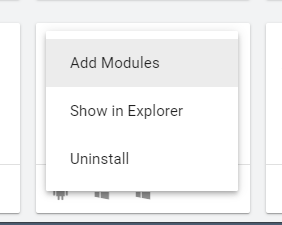
\includegraphics[width=0.6\textwidth]{img/hub3}
\caption{Se muestra la forma de acceder a la instalación de módulos.}
\end{figure}\label{fig13}
\imagen{hub2}{Se muestra la ventana para añadir los módulos.} 


\section{Compilación, instalación y ejecución del proyecto} \label{pepe}

Una vez instaladas todas las herramientas necesarias procederemos seguir los pasos para a la instalación y ejecución del proyecto. La generación de las \textit{buidls} se dividirá en 2 guías, una para cada aplicación.

El primer paso por realizar es abrir Unity Hub. Pulsamos en el botón \textit{add} y seleccionamos la carpeta principal del directorio del proyecto. Una vez seleccionado el proyecto nos aseguramos de seleccionar la versión de Unity correcta y abrimos el proyecto.

\imagen{unityhub}{Se muestra la ventana de Unity Hub donde seleccionamos la version correcta para iniciar el proyecto.}


\subsection{Ordenador}

Para configurar la aplicación del ordenador lo primero que debemos hacer es abrir su escena. Nos vamos la ventana de \textit{Project}, buscamos la carpeta \textit{Scenes} y hacemos doble clic sobre la escena con el nombre “video chat PC”.

\imagen{escenas}{Se muestra directorio del proyecto y la carpeta con las escenas}

Tras abrir la escena nos dirigiremos a la jerarquía de la escena y buscaremos el \textit{gameObject} con el nombre “Conexión”.

\imagen{jerarquiaordenador}{Se muestra jerarquía de la escena de la aplicación del ordenador.}

Haremos clic en el \textit{gameObject} y nos dirigiremos a la ventana del inspector. Ahí modificaremos el campo “http server addres” y lo cambiaremos por la \textit{IP} local de nuestro ordenador.

\imagen{2021-06-09 09_55_33-Window}{Se muestra la ventana de inspector del \textit{gameObject} “Conexión”.}

Por último, nos iremos a la ventana de \textit{File} y pulsaremos \textit{Build settings}. Ahí nos aseguraremos de que la escena cargada sea la del ordenador y que la plataforma utilizada para realizar la \textit{build} sea Pc, Mac \& Linux Standalone. Una vez realizadas las comprobaciones pulsaremos el botón de \textit{build} y elegiremos la carpeta de destino.

\begin{figure}
\centering
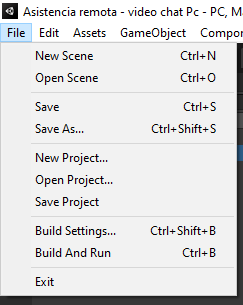
\includegraphics[width=0.3\textwidth]{img/buildsettings}
\caption{Se muestra la ventana de File y la opcion de \textit{build} settings.}
\end{figure}

\imagen{buildordenador}{Se muestra la ventana de para hacer \textit{builds} y toda su configuración}

Para ejecutar la aplicación simplemente deberemos dirigirnos a la carpeta de destino y ejecutaremos el fichero con la terminación .exe.

\subsection{HoloLens 2}

Comenzaremos abriendo la escena de “Hololens final” de la carpeta de \textit{Scene}. Nos dirigiremos a la jerarquía de la escena y buscaremos el textit{gameObject} con el nombre de “Conexión”.

\imagen{jerarquiahololens}{Se muestra jerarquía de la escena de la aplicación de las HoloLEns 2.}

Al igual que en la configuración de la aplicación del ordenador nos dirigiremos al la ventana del inspector y modificaremos el campo “http server addres” por la dirección \textit{IP} local de nuestro ordenador.

Posteriormente iremos a la ventana de \textit{Build settings} y esta vez seleccionaremos la opción de “Windows Universal Platform”. Pulsaremos el botón de \textit{Switch platform}. Una vez finalice los cambios borraremos la escena de la aplicación del ordenador y pulsaremos el botón de \textit{Add open scenes}.

\imagen{switch}{Se muestra la ventana de para hacer \textit{builds} sin haber cambiado de plataforma.}

Sin modificar ningún de valor de la configuración pulsaremos el botón de \textit{build} y seleccionaremos la carpeta de destino.

\imagen{buildhololens}{Se muestra la ventana de para hacer \textit{builds} después de cambiar la plataforma y la escena.}

Nos dirigiremos al directorio de destino y ejecutaremos con Visual Studio 2019 el archivo “Asistencia Remota.sln”

\imagen{visual}{Se muestra el directorio con la \textit{build}}

Seleccionamos el desplegable de “Máquina remota” y hacemos clic en el apartado de propiedades.

\imagen{configuracion}{Se muestra el desplegable con las diferentes opciones de compilación.}

Vamos a “Propiedades de depuración” -> “Depuracion” -> “Nombre del equipo” y modificamos el valor con la dirección \textit{IP} local de las Hololens 2.
\imagen{configuracion2}{Se muestra la ventana con las propiedades de la depuración.}

Por último, nos aseguramos de que estén seleccionadas las opciones de “Master” y “ARM” y pulsamos el botón verde del \textit{play}.

\imagen{instalacion}{Se muestra las opciones de depuración.}

